\begin{pages}
    \begin{Rightside}
    \selectlanguage{greek}
        \beginnumbering
        \pstart[
        			\chapter{Ἡ πεσοῦσα Βαβυλών}
        			\markboth{The Fallen Babylon}
				]
		\renewcommand{\LettrineFontHook}{\PHtitl}
		\lettrine[lines=3]{Μ}{ετὰ} ταῦτα εἶδον ἄλλον ἄγγελον καταβαίνοντα ἐκ τοῦ οὐρανοῦ, ἔχοντα ἐξουσίαν μεγάλην, καὶ ἡ γῆ ἐφωτίσθη ἐκ τῆς δόξης αὐτοῦ. καὶ ἔκραξεν ἐν ἰσχυρᾷ φωνῇ λέγων Ἔπεσεν ἔπεσεν Βαβυλὼν ἡ μεγάλη, καὶ ἐγένετο κατοικητήριον δαιμονίων καὶ φυλακὴ παντὸς πνεύματος ἀκαθάρτου καὶ φυλακὴ παντὸς ὀρνέου ἀκαθάρτου καὶ μεμισημένου, ὅτι ἐκ τοῦ οἴνου τοῦ θυμοῦ τῆς πορνείας αὐτῆς πέπωκαν πάντα τὰ ἔθνη, καὶ οἱ βασιλεῖς τῆς γῆς μετ’ αὐτῆς ἐπόρνευσαν, καὶ οἱ ἔμποροι τῆς γῆς ἐκ τῆς δυνάμεως τοῦ στρήνους αὐτῆς ἐπλούτησαν. 
		\pend
		\pstart
		Καὶ ἤκουσα ἄλλην φωνὴν ἐκ τοῦ οὐρανοῦ λέγουσαν Ἐξέλθατε ὁ λαός μου ἐξ αὐτῆς, ἵνα μὴ συνκοινωνήσητε ταῖς ἁμαρτίαις αὐτῆς, καὶ ἐκ τῶν πληγῶν αὐτῆς ἵνα μὴ λάβητε· ὅτι ἐκολλήθησαν αὐτῆς αἱ ἁμαρτίαι ἄχρι τοῦ οὐρανοῦ, καὶ ἐμνημόνευσεν ὁ Θεὸς τὰ ἀδικήματα αὐτῆς. ἀπόδοτε αὐτῇ ὡς καὶ αὐτὴ ἀπέδωκεν, καὶ διπλώσατε τὰ διπλᾶ κατὰ τὰ ἔργα αὐτῆς· ἐν τῷ ποτηρίῳ ᾧ ἐκέρασεν κεράσατε αὐτῇ διπλοῦν· 
		\pend
		\pstart
		ὅσα ἐδόξασεν αὐτὴν καὶ ἐστρηνίασεν, τοσοῦτον δότε αὐτῇ βασανισμὸν καὶ πένθος. ὅτι ἐν τῇ καρδίᾳ αὐτῆς λέγει ὅτι Κάθημαι βασίλισσα καὶ χήρα οὐκ εἰμί, καὶ πένθος οὐ μὴ ἴδω· διὰ τοῦτο ἐν μιᾷ ἡμέρᾳ ἥξουσιν αἱ πληγαὶ αὐτῆς, θάνατος καὶ πένθος καὶ λιμός, καὶ ἐν πυρὶ κατακαυθήσεται· ὅτι ἰσχυρὸς Κύριος ὁ Θεὸς ὁ κρίνας αὐτήν. 
		\pend
		\pstart
		καὶ κλαύσουσιν καὶ κόψονται ἐπ’ αὐτὴν οἱ βασιλεῖς τῆς γῆς οἱ μετ’ αὐτῆς πορνεύσαντες καὶ στρηνιάσαντες, ὅταν βλέπωσιν τὸν καπνὸν τῆς πυρώσεως αὐτῆς, ἀπὸ μακρόθεν ἑστηκότες διὰ τὸν φόβον τοῦ βασανισμοῦ αὐτῆς, λέγοντες Οὐαὶ οὐαί, ἡ πόλις ἡ μεγάλη, Βαβυλὼν ἡ πόλις ἡ ἰσχυρά, ὅτι μιᾷ ὥρᾳ ἦλθεν ἡ κρίσις σου. 
		\pend
		\pstart
		καὶ οἱ ἔμποροι τῆς γῆς κλαίουσιν καὶ πενθοῦσιν ἐπ’ αὐτήν, ὅτι τὸν γόμον αὐτῶν οὐδεὶς ἀγοράζει οὐκέτι, γόμον χρυσοῦ καὶ ἀργύρου καὶ λίθου τιμίου καὶ μαργαριτῶν καὶ βυσσίνου καὶ πορφύρας καὶ σιρικοῦ καὶ κοκκίνου, καὶ πᾶν ξύλον θύϊνον καὶ πᾶν σκεῦος ἐλεφάντινον καὶ πᾶν σκεῦος ἐκ ξύλου τιμιωτάτου καὶ χαλκοῦ καὶ σιδήρου καὶ μαρμάρου, καὶ κιννάμωμον καὶ ἄμωμον καὶ θυμιάματα καὶ μύρον καὶ λίβανον καὶ οἶνον καὶ ἔλαιον καὶ σεμίδαλιν καὶ σῖτον καὶ κτήνη καὶ πρόβατα, καὶ ἵππων καὶ ῥεδῶν καὶ σωμάτων, καὶ ψυχὰς ἀνθρώπων. 
		\pend
		\pstart
		καὶ ἡ ὀπώρα σου τῆς ἐπιθυμίας τῆς ψυχῆς ἀπῆλθεν ἀπὸ σοῦ, καὶ πάντα τὰ λιπαρὰ καὶ τὰ λαμπρὰ ἀπώλετο ἀπὸ σοῦ, καὶ οὐκέτι οὐ μὴ αὐτὰ εὑρήσουσιν. 
		\pend
		\pstart
		οἱ ἔμποροι τούτων, οἱ πλουτήσαντες ἀπ’ αὐτῆς, ἀπὸ μακρόθεν στήσονται διὰ τὸν φόβον τοῦ βασανισμοῦ αὐτῆς κλαίοντες καὶ πενθοῦντες, λέγοντες Οὐαὶ οὐαί, ἡ πόλις ἡ μεγάλη, ἡ περιβεβλημένη βύσσινον καὶ πορφυροῦν καὶ κόκκινον, καὶ κεχρυσωμένη ἐν χρυσίῳ καὶ λίθῳ τιμίῳ καὶ μαργαρίτῃ, ὅτι μιᾷ ὥρᾳ ἠρημώθη ὁ τοσοῦτος πλοῦτος. 
		\pend
		\pstart
		καὶ πᾶς κυβερνήτης καὶ πᾶς ὁ ἐπὶ τόπον πλέων καὶ ναῦται καὶ ὅσοι τὴν θάλασσαν ἐργάζονται, ἀπὸ μακρόθεν ἔστησαν καὶ ἔκραζον βλέποντες τὸν καπνὸν τῆς πυρώσεως αὐτῆς λέγοντες Τίς ὁμοία τῇ πόλει τῇ μεγάλῃ; καὶ ἔβαλον χοῦν ἐπὶ τὰς κεφαλὰς αὐτῶν καὶ ἔκραζον κλαίοντες καὶ πενθοῦντες, λέγοντες Οὐαὶ οὐαί, ἡ πόλις ἡ μεγάλη, ἐν ᾗ ἐπλούτησαν πάντες οἱ ἔχοντες τὰ πλοῖα ἐν τῇ θαλάσσῃ ἐκ τῆς τιμιότητος αὐτῆς, ὅτι μιᾷ ὥρᾳ ἠρημώθη. Εὐφραίνου ἐπ’ αὐτῇ, οὐρανέ καὶ οἱ ἅγιοι καὶ οἱ ἀπόστολοι καὶ οἱ προφῆται, ὅτι ἔκρινεν ὁ Θεὸς τὸ κρίμα ὑμῶν ἐξ αὐτῆς. 
		\pend
		\pstart
		Καὶ ἦρεν εἷς ἄγγελος ἰσχυρὸς λίθον ὡς μύλινον μέγαν, καὶ ἔβαλεν εἰς τὴν θάλασσαν λέγων Οὕτως ὁρμήματι βληθήσεται Βαβυλὼν ἡ μεγάλη πόλις, καὶ οὐ μὴ εὑρεθῇ ἔτι. καὶ φωνὴ κιθαρῳδῶν καὶ μουσικῶν καὶ αὐλητῶν καὶ σαλπιστῶν οὐ μὴ ἀκουσθῇ ἐν σοὶ ἔτι, καὶ πᾶς τεχνίτης πάσης τέχνης οὐ μὴ εὑρεθῇ ἐν σοὶ ἔτι, καὶ φωνὴ μύλου οὐ μὴ ἀκουσθῇ ἐν σοὶ ἔτι, καὶ φῶς λύχνου οὐ μὴ φάνῃ ἐν σοὶ ἔτι, καὶ φωνὴ νυμφίου καὶ νύμφης οὐ μὴ ἀκουσθῇ ἐν σοὶ ἔτι· ὅτι οἱ ἔμποροί σου ἦσαν οἱ μεγιστᾶνες τῆς γῆς, ὅτι ἐν τῇ φαρμακίᾳ σου ἐπλανήθησαν πάντα τὰ ἔθνη, καὶ ἐν αὐτῇ αἷμα προφητῶν καὶ ἁγίων εὑρέθη καὶ πάντων τῶν ἐσφαγμένων ἐπὶ τῆς γῆς.				
		\pend
        \endnumbering
    \end{Rightside}
    \begin{Leftside}
        \beginnumbering
        \pstart[
        			\chapter{The Fallen Babylon}
				]		
				
		\renewcommand{\LettrineFontHook}{\Zallmanfamily}
		\lettrine[lines=3]{A}{fter} this I saw another angel coming down from Heaven, having (a) great authority; and the Earth was illuminated through his glory. And he shouted in a strong voice saying, “The great (city of) Babylon, it fell, it fell. And it became (was) a dwelling place of demons and a prison of every unclean spirit and a prison of every unclean and hateful bird; for from the wine of the wrath of her sexual immorality have drunk all the nations, and the kings of the Earth committed adultery with her and the merchants of the Earth became rich from the power of her sensuality (luxury). 
		\pend
		\pstart
		And I heard another voice from Heaven saying, “Come out of her, my people, so that you may not share in her sins and so that you may not take (receive) (anything) from her plagues (so that you may not get infected with her plagues). For her sins have combined (and piled up) into Heaven and God remembered her wrongdoings. Give her back (sell her) as she has also given back (sold) and double the double (double it?) according to her deeds. In the cup which she mixed, mixed her double (make twice as much as she made). 
		\pend
		\pstart
		As many (people as there were who) glorified her and (as many as) lived sensually (with her), that many (people) (will) give her torment and mourning. For in her heart she says that “I am sitting (as a) queen and I am not a widow; and I do not see (any) mourning.” Because of this there will one day come her plagues — death and mourning and famine — and she will be burned (up) in fire; for the Lord God, her judge, is strong. 
		\pend
		\pstart
		And the kings of the Earth — those who committed adultery with her and lived in sensuality (with her) — will weep and strike (at) her when they see the smoke of her burning (up). (And they are) standing far away through (because of) the fear (in fear) of her torment saying, “Woe, woe (to you) O great and strong city Babylon; for in one (single) hour has come your judgement.”
		\pend
		\pstart
		And the merchants of the Earth will weep and mourn (at) her, for nobody buys their goods anymore. Their golden and silver goods and (their goods made out of) precious stone and pearls and (their goods) made out of fine linen and purple cloth and silk and scarlet; and every scented tree and every item made out of ivory and every item made out of costly wood and brass and iron and marble. And (also their) cinnamon and spice and incense and myrrh and frankincense and wine and olive oil and fine flour and wheat; and (their) cattle and sheep and horses and chariots and bodies (slaves?) and human souls. 
		\pend
		\pstart
		“And the ripe fruit of your soul’s lust (the ripe fruit your soul longs for) has departed from you and all the things (you held) precious and (that were) luxurious, they (also) departed from you — and they will never (again) find them (you will not find them again).” 
		\pend
		\pstart
		And the merchants of these (goods) — those (merchants) who became rich (by selling her things) — they are standing far away because of the fear of (i. e. fearing) her torment (and they are) weeping and mourning saying, “Woe woe (to you), O great city clothed in fine purple and scarlet linen and adorned with gold and precious stone and pearls — for in one (single) hour your great wealth has been made desolate.”
		\pend
		\pstart
		And every captain and every sea traveller and (every) seaman (sailor) and whosoever works at the sea — they are (all) standing far away and they shouted seeing the smoke of her burning (up) saying, “Who (what) is alike the great city?” And they threw dust onto their heads and they shouted (whilst they were) weeping and mourning (and they were) saying, “Woe, woe (to you), O great city in which (through which) were made rich all those who have ships in the sea through her wealth; for in one (single) hour she has been laid waste.” Rejoice over her, O Heaven and (you) holy men and apostles and prophets; for God has judged your judgment from her (God avenged you?). 
		\pend
		\pstart
		And one strong angel picked up a stone — like a great millstone — and threw it into the sea saying, “Thus with wrath (anger) Babylon — the great city — will be cast down; and it will no longer be found. And the sound of harpists and musicians and flute players and trumpeters will not be heard in you any longer, nor will any craftsmen of any craft be found in you any longer, nor will the voice of a mill be heard in you any longer. And the light of a lamp shall not shine in you any longer, nor shall the voice(s) of a bridegroom or a bride be heard in you any longer; for your merchants were the great (ones) of the Earth (and) for all nations were deceived by your sorcery (magic). And in her the blood of (the) prophets and saints was found, and (also that) of every slain (one) upon the Earth.” 
		\pend
        \endnumbering
    \end{Leftside}

\end{pages} 
\Pages

\clearpage
\thispagestyle{empty}
\null\vfill
\settowidth\longest{\huge\itshape […] and when I turned around I saw}
\begin{center}
\parbox{\longest}{%
  \raggedright{\huge\itshape%
    ``The great Babylon, it fell, it fell.'' \par\bigskip
  }
  \raggedleft\Large\MakeUppercase{``Babylon Fallen'' — Gustave Doré, 1866}\par%
}
\vfill\vfill
\clearpage\newpage
\end{center}
\newpage
\thispagestyle{empty}
\begin{center}
	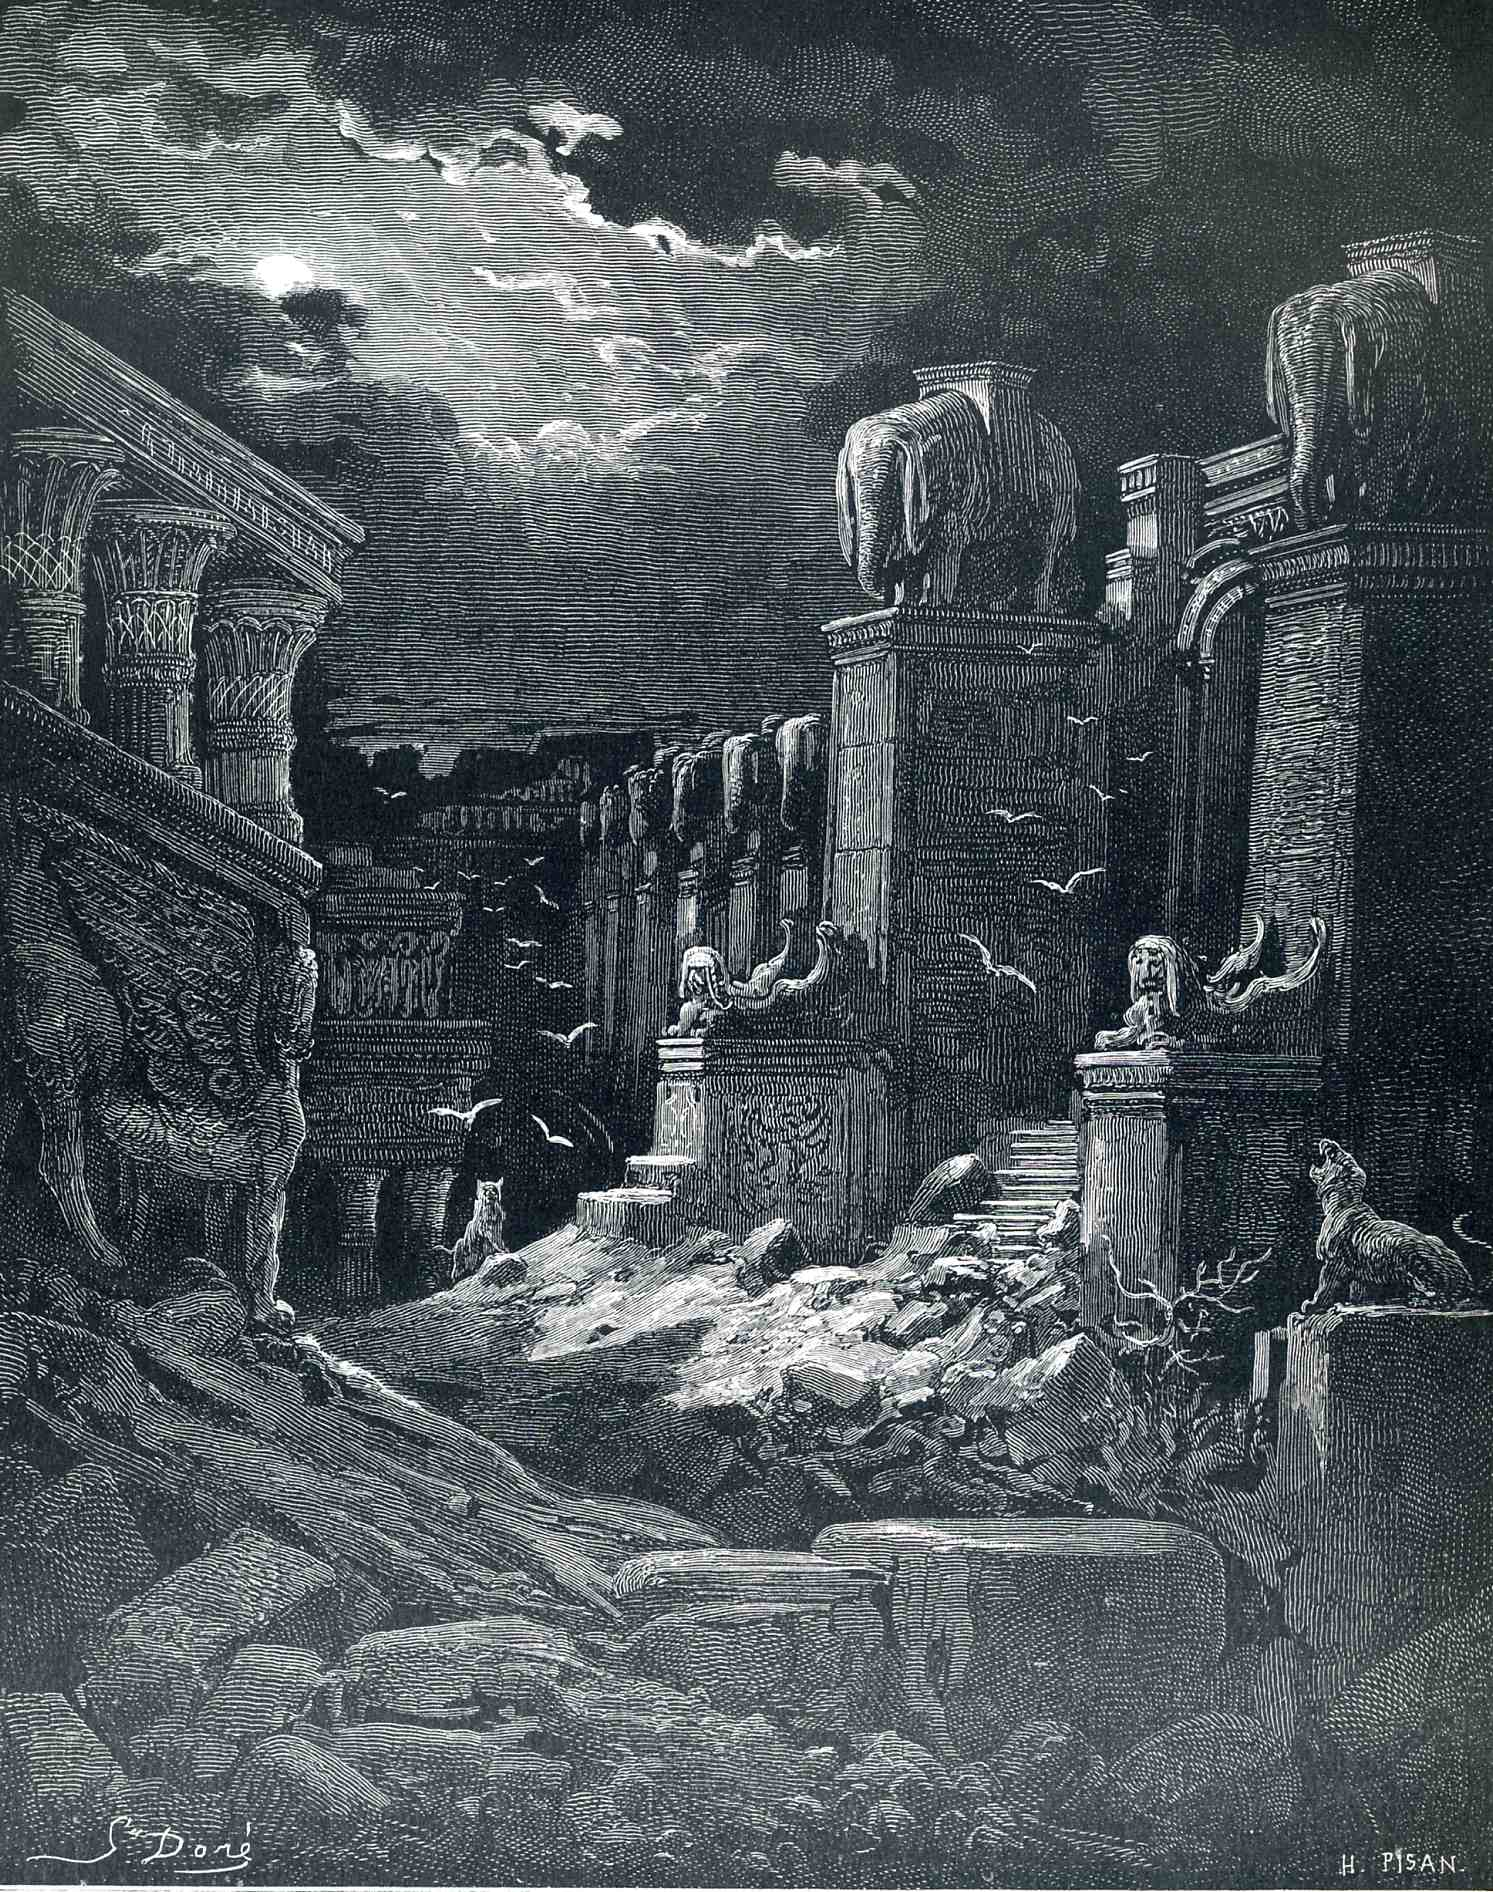
\includegraphics[width=1\textwidth]{images/illustrations/dorebabylon}
\end{center}